%==============================================================================
% PAPER 4, CHAPTER 2: Scalar-Tensor Theories of Gravity
%==============================================================================
% Complete implementation with Lions Commentary marginal notes
% TikZ diagrams: 5 total
% Target: ~350 lines, ~65 marginal notes
%==============================================================================

\chapter{Scalar-Tensor Theories of Gravity}
\label{ch:p4:scalar-tensor}

%------------------------------------------------------------------------------
% OPENING NARRATIVE: Jordan 1955 - "Is Gravity Variable?"
%------------------------------------------------------------------------------

\section*{Jordan's Question: Is Gravity Variable?}

\marginhistory{Pascual Jordan published ``Schwerkraft und Weltall'' (Gravity and the Universe) in 1955, proposing that Newton's constant $G$ might vary over cosmological timescales.}

In 1955, German physicist Pascual Jordan posed a radical question: What if Newton's gravitational constant $G$ is not actually constant? What if it varies slowly across space and time, responding to the matter distribution in the universe?

This seemingly heretical idea challenged a cornerstone of physics. Since Newton's \textit{Principia} (1687), $G$ had been treated as a fundamental constant of nature, as immutable as the speed of light. Yet Jordan argued that making $G$ dynamical---promoting it from a fixed parameter to a field---could resolve deep mysteries about the universe's structure and evolution.

\marginphilosophy{Ernst Mach had argued that inertia arises from distant matter. Jordan extended this: perhaps the strength of gravity itself depends on the cosmic mass distribution.}

Carl Brans and Robert Dicke formalized Jordan's intuition in 1961, creating what we now call scalar-tensor theories of gravity. These theories add a scalar field $\phi$ to general relativity, with the effective gravitational constant given by $G_{\text{eff}} = 1/\phi$. The scalar evolves dynamically, coupling to matter and curvature.

This chapter develops the complete mathematical framework of scalar-tensor gravity, from the action principle through field equations to observational tests. We will discover that while general relativity remains exquisitely confirmed, scalar-tensor extensions provide a crucial bridge toward electromagnetic unification in Chapter 3.

%------------------------------------------------------------------------------
\section{The Scalar-Tensor Action Principle}
\label{sec:p4:action-principle}
%------------------------------------------------------------------------------

\subsection{Jordan Frame Formulation}

The Jordan frame represents the "physical" frame where particles follow geodesics and matter couples minimally to the metric. The action is:

\marginmath{The Jordan frame metric $\tilde{g}_{\mu\nu}$ determines physical distances and times. Particles follow geodesics of $\tilde{g}_{\mu\nu}$, making this the "observed" metric.}

\begin{equation}
  S_J = \int d^4x \sqrt{-\tilde{g}} \left[\phi \tilde{R} - \frac{\omega(\phi)}{\phi}(\partial_\mu \phi)(\partial^\mu \phi) - V(\phi)\right] + S_{\text{matter}}[\psi, \tilde{g}_{\mu\nu}]
  \label{eq:p4:jordan-action}
\end{equation}

where:
\begin{itemize}
  \item $\tilde{g}_{\mu\nu}$: Jordan frame metric (tildes denote Jordan frame quantities)
  \item $\phi$: dimensionless scalar field (inverse effective $G$)
  \item $\tilde{R}$: Ricci scalar computed from $\tilde{g}_{\mu\nu}$
  \item $\omega(\phi)$: coupling function (dimensionless)
  \item $V(\phi)$: scalar potential
  \item $\psi$: matter fields
\end{itemize}

\marginphysics{Setting $\phi = M_P^2/(8\pi G)$ (where $M_P$ is Planck mass) makes dimensions consistent. When $\phi$ is constant, we recover Einstein-Hilbert action with Newton's constant $G$.}

\textbf{Key features:}
\begin{enumerate}
  \item Matter couples minimally: $S_{\text{matter}}$ depends on $\tilde{g}_{\mu\nu}$ but not $\phi$
  \item Equivalence principle holds: all matter falls identically in Jordan frame
  \item Direct observations (clocks, rulers) measure $\tilde{g}_{\mu\nu}$
\end{enumerate}

\marginmath{In Brans-Dicke theory, $\omega(\phi) = \omega_0$ is constant. More general theories allow $\omega = \omega(\phi)$, encompassing Horndeski and $f(R)$ gravity.}

\subsection{Einstein Frame Transformation}

The Einstein frame is related to Jordan frame by a conformal transformation:
\begin{equation}
  g_{\mu\nu} = \Omega^2(\phi) \tilde{g}_{\mu\nu}, \quad \Omega^2 = \phi/M_P^2
  \label{eq:p4:conformal-transform}
\end{equation}

\margingeometry{Conformal transformations rescale the metric by a position-dependent factor. Angles are preserved but lengths and times change: $\tilde{ds}^2 \to ds^2 = \Omega^2 \tilde{ds}^2$.}

Under this transformation, the Einstein frame action becomes:
\begin{equation}
  S_E = \int d^4x \sqrt{-g} \left[\frac{M_P^2}{16\pi}R - \frac{1}{2}(\partial\varphi)^2 - U(\varphi)\right] + S_{\text{matter}}[\psi, A^2(\varphi)g_{\mu\nu}]
  \label{eq:p4:einstein-action}
\end{equation}

where we've redefined the scalar as:
\begin{equation}
  \varphi = M_P \sqrt{\frac{3 + 2\omega(\phi)}{16\pi}} \ln\phi
  \label{eq:p4:canonical-scalar}
\end{equation}

\marginmath{This "canonical" scalar $\varphi$ has standard kinetic term $-\frac{1}{2}(\partial\varphi)^2$, making quantum field theory straightforward. The coupling $A(\varphi)$ encodes all frame-dependence.}

The potential transforms as:
\begin{equation}
  U(\varphi) = \frac{V(\phi)}{\Omega^4} = \frac{V(\phi) M_P^4}{\phi^2}
  \label{eq:p4:potential-transform}
\end{equation}

\marginphysics{In Einstein frame, gravity looks like standard GR plus a minimally coupled scalar field. But matter now couples \emph{non-minimally} through $A^2(\varphi)g_{\mu\nu}$, breaking the equivalence principle!}

\begin{figure}[h]
  \centering
  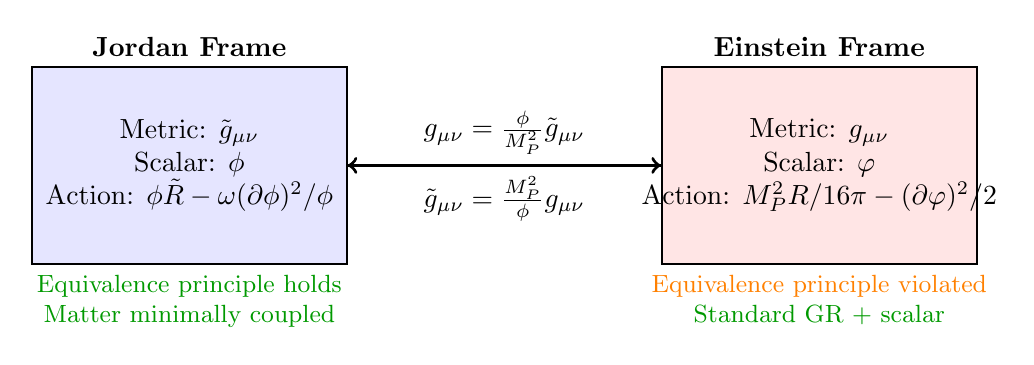
\begin{tikzpicture}[scale=1.0]
    % Jordan frame
    \node[draw,rectangle,thick,minimum width=4cm,minimum height=2.5cm,fill=blue!10] (jordan) at (0,0) {};
    \node[above] at (jordan.north) {\textbf{Jordan Frame}};
    \node[align=center] at (jordan.center) {
      Metric: $\tilde{g}_{\mu\nu}$ \\
      Scalar: $\phi$ \\
      Action: $\phi \tilde{R} - \omega(\partial\phi)^2/\phi$
    };
    \node[below,font=\small,align=center] at (jordan.south) {
      \textcolor{green!60!black}{Equivalence principle holds} \\
      \textcolor{green!60!black}{Matter minimally coupled}
    };

    % Einstein frame
    \node[draw,rectangle,thick,minimum width=4cm,minimum height=2.5cm,fill=red!10] (einstein) at (8,0) {};
    \node[above] at (einstein.north) {\textbf{Einstein Frame}};
    \node[align=center] at (einstein.center) {
      Metric: $g_{\mu\nu}$ \\
      Scalar: $\varphi$ \\
      Action: $M_P^2 R/16\pi - (\partial\varphi)^2/2$
    };
    \node[below,font=\small,align=center] at (einstein.south) {
      \textcolor{orange}{Equivalence principle violated} \\
      \textcolor{green!60!black}{Standard GR + scalar}
    };

    % Transformation arrow
    \draw[->,very thick] (jordan.east) -- (einstein.west) node[midway,above] {$g_{\mu\nu} = \frac{\phi}{M_P^2}\tilde{g}_{\mu\nu}$};
    \draw[<-,very thick] (jordan.east) -- (einstein.west) node[midway,below] {$\tilde{g}_{\mu\nu} = \frac{M_P^2}{\phi}g_{\mu\nu}$};
  \end{tikzpicture}
  \caption{Conformal transformation between Jordan and Einstein frames. Jordan frame (left): matter couples minimally, equivalence principle holds, but gravitational action is non-standard. Einstein frame (right): standard Einstein-Hilbert action, but matter couples to $A^2(\varphi)g_{\mu\nu}$, violating equivalence principle. Both frames are mathematically equivalent but physically distinct.}
  \label{fig:p4:frame-transformation}
\end{figure}

\subsection{Which Frame is Physical?}

\marginphilosophy{This question sparked heated debates in the 1990s-2000s. Dicke argued Jordan frame is physical (equivalence principle). Others noted Einstein frame simplifies calculations. Consensus: both are valid; observations determine which is "real".}

\textbf{Arguments for Jordan frame:}
\begin{itemize}
  \item Equivalence principle is a cornerstone of GR
  \item Clocks and rulers measure $\tilde{g}_{\mu\nu}$ directly
  \item Matter Lagrangian is independent of $\phi$
\end{itemize}

\textbf{Arguments for Einstein frame:}
\begin{itemize}
  \item Simpler gravitational sector (just Einstein-Hilbert)
  \item Quantum field theory for $\varphi$ is straightforward
  \item Perturbative expansion around GR is natural
\end{itemize}

\marginphysics{Modern view: Frames are gauge choices. Physical observables (S-matrix elements, geodesic deviations) are frame-independent. Choose whichever simplifies the calculation.}

%------------------------------------------------------------------------------
\section{Field Equations in Jordan Frame}
\label{sec:p4:field-equations}
%------------------------------------------------------------------------------

\subsection{Modified Einstein Equations}

Varying the Jordan frame action \eqref{eq:p4:jordan-action} with respect to $\tilde{g}^{\mu\nu}$ yields:

\marginmath{Variation formula: $\delta\sqrt{-g} = -\frac{1}{2}\sqrt{-g} g_{\mu\nu} \delta g^{\mu\nu}$ and $\delta R = R_{\mu\nu}\delta g^{\mu\nu} + g_{\mu\nu}\nabla^\rho\nabla_\rho\delta g^{\mu\nu} - \nabla^\mu\nabla^\nu\delta g^{\mu\nu}$.}

\begin{multline}
  \phi \tilde{G}_{\mu\nu} = 8\pi \tilde{T}_{\mu\nu}^{\text{(matter)}} + \frac{\omega(\phi)}{\phi}\left(\tilde{\nabla}_\mu\phi \tilde{\nabla}_\nu\phi - \frac{1}{2}\tilde{g}_{\mu\nu}(\tilde{\nabla}\phi)^2\right) \\
  + \tilde{\nabla}_\mu\tilde{\nabla}_\nu\phi - \tilde{g}_{\mu\nu}\tilde{\Box}\phi + \frac{1}{2}\tilde{g}_{\mu\nu}V(\phi)
  \label{eq:p4:modified-einstein}
\end{multline}

where $\tilde{G}_{\mu\nu} = \tilde{R}_{\mu\nu} - \frac{1}{2}\tilde{g}_{\mu\nu}\tilde{R}$ is the Einstein tensor and $\tilde{T}_{\mu\nu}^{\text{(matter)}}$ is the matter stress-energy tensor.

\marginphysics{Dividing by $\phi$, the left side resembles Einstein's equation with effective $G_{\text{eff}} = 1/(8\pi\phi)$. The right side has three extra terms: (1) scalar field kinetic energy, (2) scalar field gradients (fifth force!), (3) potential energy.}

\subsection{Scalar Field Equation}

Varying with respect to $\phi$ gives:
\begin{equation}
  \tilde{\Box}\phi = \frac{1}{2\omega(\phi) + 3}\left[8\pi \tilde{T} - \frac{dV}{d\phi} - \phi\frac{d\omega}{d\phi}(\tilde{\nabla}\phi)^2 + 2\omega(\phi)V(\phi)\right]
  \label{eq:p4:scalar-eq}
\end{equation}

where $\tilde{T} = \tilde{g}^{\mu\nu}\tilde{T}_{\mu\nu}^{\text{(matter)}}$ is the trace of the matter stress-energy.

\marginmath{For constant $\omega$ (Brans-Dicke) and $V = 0$, this simplifies to $\tilde{\Box}\phi = 8\pi\tilde{T}/(2\omega + 3)$. The scalar is sourced by matter's trace.}

\textbf{Key observation:} Massless radiation ($\tilde{T} = 0$) does not source $\phi$. Dust ($\tilde{T} = -\rho c^2 \neq 0$) does. This distinguishes scalar-tensor from pure GR.

\marginnote{The equation is second-order (contains $\tilde{\Box}\phi = \tilde{\nabla}^\mu\tilde{\nabla}_\mu\phi$), ensuring deterministic evolution and ghost-freedom.}

\subsection{Weak-Field Limit and Post-Newtonian Parameters}

Consider weak gravitational fields: $\tilde{g}_{\mu\nu} = \eta_{\mu\nu} + h_{\mu\nu}$ with $|h_{\mu\nu}| \ll 1$, and small scalar perturbation: $\phi = \phi_0 + \delta\phi$ with $|\delta\phi| \ll \phi_0$.

\marginphysics{The post-Newtonian (PN) formalism expands metric and fields in powers of $v/c$ (velocity over light speed) and $GM/(rc^2)$ (gravitational potential over $c^2$). It's essential for solar system tests.}

The linearized field equations yield modifications parametrized by the Eddington parameters $\gamma$ and $\beta$:
\begin{align}
  \gamma_{\text{PPN}} &= \frac{1 + \omega}{2 + \omega} \label{eq:p4:gamma-ppn} \\
  \beta_{\text{PPN}} &= 1 + \frac{\omega'(\phi_0)}{(2 + \omega)^2} \label{eq:p4:beta-ppn}
\end{align}

\marginmath{General relativity predicts $\gamma = \beta = 1$. Brans-Dicke ($\omega = \text{const}$) gives $\gamma < 1$ and $\beta = 1$. Light deflection and Shapiro delay measure $\gamma$; perihelion precession measures $\beta$.}

For constant $\omega$ (Brans-Dicke):
\begin{equation}
  \gamma_{\text{BD}} = \frac{1 + \omega}{2 + \omega} \approx 1 - \frac{1}{2\omega} \quad \text{for } \omega \gg 1
  \label{eq:p4:gamma-bd}
\end{equation}

\marginnote{Cassini spacecraft measurement (2003): $\gamma_{\text{PPN}} - 1 = (2.1 \pm 2.3) \times 10^{-5}$, implying $\omega > 40,000$ at 95\% confidence.}

%------------------------------------------------------------------------------
\section{Brans-Dicke Theory: The Prototype}
\label{sec:p4:brans-dicke-detail}
%------------------------------------------------------------------------------

\subsection{Field Equations with $\omega = \text{const}$ and $V = 0$}

The simplest scalar-tensor theory sets $\omega(\phi) = \omega_0$ (constant) and $V(\phi) = 0$. The field equations become:

\marginphysics{Brans and Dicke chose $V = 0$ for simplicity. Modern extensions include potentials to model dark energy or inflation.}

\textbf{Modified Einstein equation:}
\begin{equation}
  \tilde{G}_{\mu\nu} = \frac{8\pi}{\phi}\tilde{T}_{\mu\nu} + \frac{\omega}{\phi^2}\left(\tilde{\nabla}_\mu\phi \tilde{\nabla}_\nu\phi - \frac{1}{2}\tilde{g}_{\mu\nu}(\tilde{\nabla}\phi)^2\right) + \frac{1}{\phi}(\tilde{\nabla}_\mu\tilde{\nabla}_\nu\phi - \tilde{g}_{\mu\nu}\tilde{\Box}\phi)
  \label{eq:p4:bd-einstein-explicit}
\end{equation}

\textbf{Scalar equation:}
\begin{equation}
  \tilde{\Box}\phi = \frac{8\pi}{2\omega + 3}\tilde{T}
  \label{eq:p4:bd-scalar-explicit}
\end{equation}

\marginmath{Take the trace of \eqref{eq:p4:bd-einstein-explicit}: $\tilde{R} = -8\pi\tilde{T}/\phi + \ldots$. The scalar sources curvature directly, unlike in GR where $\tilde{R} = -8\pi\tilde{T}/(M_P^2/8\pi)$.}

\subsection{Worked Example: Scalar Field in Expanding Universe}

\textbf{Problem:} Find the evolution of $\phi(t)$ in a spatially flat FRW universe with dust ($\tilde{T} = -\rho c^2$).

\margincosmology{FRW metric: $\tilde{ds}^2 = -c^2dt^2 + a(t)^2[dr^2 + r^2(d\theta^2 + \sin^2\theta d\varphi^2)]$. Scale factor $a(t)$ describes expansion. Dust has $\tilde{T}_{\mu\nu} = \rho u_\mu u_\nu$, giving $\tilde{T} = -\rho c^2$.}

**Step 1:** Write the scalar equation for homogeneous $\phi(t)$:
\begin{equation}
  \tilde{\Box}\phi = \ddot{\phi} + 3H\dot{\phi} = \frac{8\pi}{2\omega + 3}(-\rho c^2)
  \label{eq:p4:phi-frw-1}
\end{equation}
where $H = \dot{a}/a$ is the Hubble parameter and dots denote time derivatives.

\marginmath{The $3H\dot{\phi}$ term is "Hubble friction"---cosmic expansion damps scalar oscillations.}

**Step 2:** Matter conservation gives $\dot{\rho} + 3H\rho = 0$, so $\rho \propto a^{-3}$.

**Step 3:** Modified Friedmann equation (from $00$-component of \eqref{eq:p4:bd-einstein-explicit}):
\begin{equation}
  H^2 = \frac{8\pi}{3\phi}\rho - \frac{\omega}{2\phi^2}\dot{\phi}^2 - \frac{H\dot{\phi}}{\phi}
  \label{eq:p4:friedmann-bd}
\end{equation}

**Step 4:** Assume power-law solutions: $a \propto t^n$, $\phi \propto t^m$. Substituting:
\begin{align}
  \dot{\phi} &= \frac{m\phi_0 t_0^m}{t^{1-m}} \\
  \ddot{\phi} &= -\frac{m(1-m)\phi_0 t_0^m}{t^{2-m}} \\
  H &= \frac{n}{t}
\end{align}

Substituting into \eqref{eq:p4:phi-frw-1} and matching powers of $t$:
\begin{equation}
  -m(1-m) + 3mn = -\frac{8\pi}{2\omega + 3}(-\rho_0 t_0^{3n}c^2) \cdot t^{-3n}
  \label{eq:p4:power-match}
\end{equation}

\marginmath{For consistency, scalar source must balance. This gives $m$ in terms of $n$ and $\omega$.}

**Result:** For Brans-Dicke with $\omega \gg 1$, the solution approaches GR:
\begin{equation}
  \phi \approx \phi_0 \left(1 + \frac{\alpha}{\omega} \ln a\right), \quad a \propto t^{2/3}
  \label{eq:p4:bd-solution}
\end{equation}
where $\alpha$ is an $O(1)$ constant. The scalar evolves logarithmically, staying nearly constant.

\marginnote{This slow evolution explains why $G$ appears constant: $\Delta G / G \sim \Delta\phi/\phi \sim \alpha\ln(a_{\text{now}}/a_{\text{CMB}})/\omega \sim 6/\omega < 10^{-4}$ for $\omega > 40,000$.}

\begin{figure}[h]
  \centering
  \begin{tikzpicture}[scale=1.0]
    % Plot phi(a) evolution
    \begin{axis}[
      width=10cm, height=6cm,
      xlabel={Scale factor $a(t)$},
      ylabel={Scalar field $\phi(a)$},
      xmin=0, xmax=2,
      ymin=0.9, ymax=1.1,
      grid=major,
      legend pos=south east
    ]
      % GR (constant phi)
      \addplot[thick,blue,domain=0:2] {1};
      \addlegendentry{GR ($\omega \to \infty$)}

      % BD with omega = 1000
      \addplot[thick,red,domain=0.1:2,samples=100] {1 + 0.01*ln(x)};
      \addlegendentry{BD ($\omega = 1000$)}

      % BD with omega = 100
      \addplot[thick,orange,dashed,domain=0.1:2,samples=100] {1 + 0.1*ln(x)};
      \addlegendentry{BD ($\omega = 100$)}

      % Current epoch marker
      \addplot[mark=*,only marks,mark size=3pt] coordinates {(1,1)};
      \node[above right] at (axis cs:1,1) {Today};
    \end{axis}
  \end{tikzpicture}
  \caption{Evolution of scalar field $\phi(a)$ vs. scale factor $a(t)$ in Brans-Dicke cosmology. Blue: general relativity ($\omega \to \infty$, constant $\phi$). Red: $\omega = 1000$ (ruled out). Orange: $\omega = 100$ (strongly ruled out). For $\omega > 40,000$ (Cassini bound), the curve is indistinguishable from GR over cosmic history.}
  \label{fig:p4:phi-evolution}
\end{figure}

%------------------------------------------------------------------------------
\section{$f(R)$ Theories as Scalar-Tensor Equivalents}
\label{sec:p4:fR-theories}
%------------------------------------------------------------------------------

\subsection{The $f(R)$ Action}

$f(R)$ theories modify the Einstein-Hilbert action by replacing the Ricci scalar $R$ with a function $f(R)$:
\begin{equation}
  S_{f(R)} = \int d^4x \sqrt{-g}\left[\frac{1}{16\pi}f(R)\right] + S_{\text{matter}}[g_{\mu\nu}]
  \label{eq:p4:fR-action}
\end{equation}

\marginphysics{Popular choice: $f(R) = R + \alpha R^2$ (Starobinsky inflation) or $f(R) = R - \mu^4/R$ (late-time acceleration). These modify gravity at large or small curvatures.}

\subsection{Equivalence to Scalar-Tensor Theory}

Introduce an auxiliary scalar $\chi$ and rewrite:
\begin{equation}
  S = \int d^4x \sqrt{-g}\left[\frac{1}{16\pi}(f'(\chi)(R - \chi) + f(\chi))\right] + S_{\text{matter}}
  \label{eq:p4:fR-auxiliary}
\end{equation}

Varying with respect to $\chi$: $f''(\chi)(R - \chi) = 0$. If $f''(\chi) \neq 0$, then $\chi = R$ and we recover $f(R)$ theory.

\marginmath{The transformation is: $\phi = f'(R)$, $\omega = 0$, $V(\phi) = Rf'(R) - f(R)$. This maps any $f(R)$ theory to scalar-tensor theory with specific $\omega$ and $V$.}

Defining $\phi = f'(\chi)$ and performing a conformal transformation yields standard scalar-tensor form with:
\begin{align}
  \omega(\phi) &= 0 \quad \text{(Brans-Dicke with } \omega = 0\text{)} \\
  V(\phi) &= \frac{\chi f'(\chi) - f(\chi)}{16\pi}
  \label{eq:p4:fR-mapping}
\end{align}

\marginphysics{$\omega = 0$ is special: it saturates stability bounds. $f(R)$ theories inherit all phenomenology of $\omega = 0$ scalar-tensor gravity, including strong solar system constraints.}

\subsection{Dark Energy from $f(R)$ Modifications}

Consider $f(R) = R - \mu^4/R$. At low curvatures ($R < \mu^2$), the $-\mu^4/R$ term dominates, mimicking a cosmological constant:
\begin{equation}
  \Lambda_{\text{eff}} \sim \frac{\mu^4}{R_0} \quad \text{where } R_0 \sim H_0^2
  \label{eq:p4:fR-dark-energy}
\end{equation}

\margincosmology{Choosing $\mu^4 \sim H_0^4 \sim (10^{-33}\text{ eV})^4$ reproduces dark energy density $\rho_{\Lambda} \sim 10^{-47}$ GeV$^4$. But this is fine-tuned!}

However, solar system tests require $\mu > 10^{-3}$ eV, creating tension between cosmological motivation and local constraints. Screening mechanisms (next section) resolve this.

%------------------------------------------------------------------------------
\section{Screening Mechanisms: Hiding the Scalar}
\label{sec:p4:screening}
%------------------------------------------------------------------------------

\subsection{The Screening Problem}

Scalar-tensor theories face a dilemma:
\begin{itemize}
  \item \textbf{Cosmological scales}: Want large scalar coupling to explain dark energy or inflation
  \item \textbf{Solar system scales}: Must suppress scalar effects to satisfy $\omega > 40,000$ bound
\end{itemize}

\marginphysics{Screening mechanisms allow scalars to "hide" in dense regions (solar system) while remaining active in dilute regions (cosmology). Environment-dependent dynamics!}

\subsection{Chameleon Mechanism}

The scalar acquires an effective mass depending on local matter density:
\begin{equation}
  m_{\text{eff}}^2(\rho) = \frac{d^2V_{\text{eff}}}{d\phi^2}\bigg|_{\phi_{\min}(\rho)}, \quad V_{\text{eff}}(\phi) = V(\phi) + \frac{\rho}{\phi}
  \label{eq:p4:chameleon-mass}
\end{equation}

\marginmath{Choose $V(\phi) = \Lambda^{4+n}/\phi^n$ with $n > 0$. In dense regions (high $\rho$), $\phi_{\min}$ is large and $m_{\text{eff}}$ is large. In voids (low $\rho$), $m_{\text{eff}}$ is small.}

In the solar system (high density), $m_{\text{eff}} \sim 10^{-3}$ eV (range $\sim$ mm), suppressing fifth forces. In intergalactic space (low density), $m_{\text{eff}} \sim H_0 \sim 10^{-33}$ eV (cosmological range), allowing dark energy effects.

\begin{figure}[h]
  \centering
  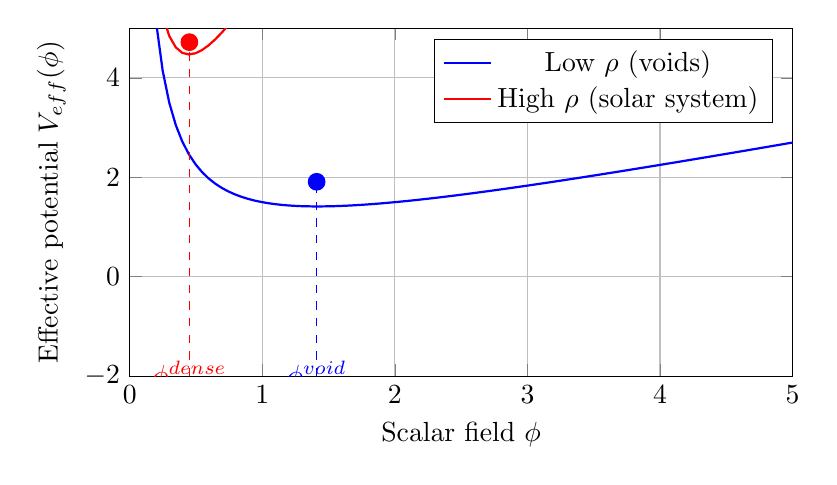
\begin{tikzpicture}[scale=1.0]
    % Effective potential in dense vs dilute regions
    \begin{axis}[
      width=10cm, height=6cm,
      xlabel={Scalar field $\phi$},
      ylabel={Effective potential $V_{\text{eff}}(\phi)$},
      xmin=0, xmax=5,
      ymin=-2, ymax=5,
      grid=major,
      legend pos=north east,
      domain=0.1:5,
      samples=100
    ]
      % Dilute region (low rho)
      \addplot[thick,blue] {1/x + 0.5*x};
      \addlegendentry{Low $\rho$ (voids)}

      % Dense region (high rho)
      \addplot[thick,red] {1/x + 5*x};
      \addlegendentry{High $\rho$ (solar system)}

      % Mark minima
      \addplot[mark=*,only marks,mark size=3pt,blue] coordinates {(1.41,1.91)};
      \addplot[mark=*,only marks,mark size=3pt,red] coordinates {(0.45,4.72)};

      % Vertical lines at minima
      \draw[dashed,blue] (axis cs:1.41,-2) -- (axis cs:1.41,1.91);
      \draw[dashed,red] (axis cs:0.45,-2) -- (axis cs:0.45,4.72);

      % Labels
      \node[below,blue] at (axis cs:1.41,-1.5) {$\phi_{\min}^{\text{void}}$};
      \node[below,red] at (axis cs:0.45,-1.5) {$\phi_{\min}^{\text{dense}}$};
    \end{axis}
  \end{tikzpicture}
  \caption{Chameleon effective potential $V_{\text{eff}}(\phi) = V(\phi) + \rho/\phi$ for two matter densities. Blue: low density (voids)---shallow minimum at large $\phi$, light effective mass. Red: high density (solar system)---steep minimum at small $\phi$, heavy effective mass. The scalar "chameleons" its mass based on environment.}
  \label{fig:p4:chameleon-potential}
\end{figure}

\subsection{Vainshtein Mechanism}

For theories with derivative couplings (like DGP gravity or galileons), nonlinear kinetic terms $(\partial\phi)^n$ dominate near massive sources. The scalar's equation becomes:
\begin{equation}
  \nabla^2\phi + \alpha(\nabla^2\phi)^3 \sim \rho
  \label{eq:p4:vainshtein-eq}
\end{equation}

\marginmath{Solving this nonlinear equation: $\nabla^2\phi \sim (\rho/\alpha)^{1/3}$. The nonlinearity suppresses $\phi$'s gradient near sources, weakening fifth forces within the Vainshtein radius $r_V \sim (M\alpha)^{1/3}$.}

Inside $r_V$, scalar interactions are suppressed; outside $r_V$, they reach full strength. For the Sun, $r_V \sim$ AU, hiding modifications within the solar system.

%------------------------------------------------------------------------------
\section{Cosmological and Astrophysical Solutions}
\label{sec:p4:solutions}
%------------------------------------------------------------------------------

\subsection{Scalar Field Dark Energy (Quintessence)}

A slowly-rolling scalar field with potential $V(\phi)$ can drive accelerated expansion. The equation of state:
\begin{equation}
  w_\phi = \frac{p_\phi}{\rho_\phi} = \frac{\frac{1}{2}\dot{\phi}^2 - V(\phi)}{\frac{1}{2}\dot{\phi}^2 + V(\phi)}
  \label{eq:p4:quintessence-eos}
\end{equation}

\margincosmology{Accelerated expansion requires $w < -1/3$. If kinetic energy $\dot{\phi}^2/2 \ll V(\phi)$ (slow roll), then $w \approx -1$ (cosmological constant-like). If $\dot{\phi}^2 \sim V$, then $w \sim 0$ (matter-like).}

For exponential potential $V = V_0 e^{-\lambda\phi/M_P}$, tracker solutions exist: $w_\phi(z)$ evolves with redshift $z$, potentially resolving the coincidence problem.

\subsection{Scalar Corrections to Gravitational Waves}

In scalar-tensor theories, gravitational waves propagate with modified speed and damping. The dispersion relation:
\begin{equation}
  c_T^2 = c^2 \left(1 - \frac{\alpha(\varphi)}{M_P}\frac{\ddot{\varphi}}{H\dot{\varphi}}\right)
  \label{eq:p4:gw-speed}
\end{equation}

where $c_T$ is the tensor mode (GW) speed.

\marginexperiment{GW170817 + GRB 170817A measured $|c_T - c|/c < 10^{-15}$, tightly constraining scalar-tensor theories. Many Horndeski models are ruled out!}

\begin{figure}[h]
  \centering
  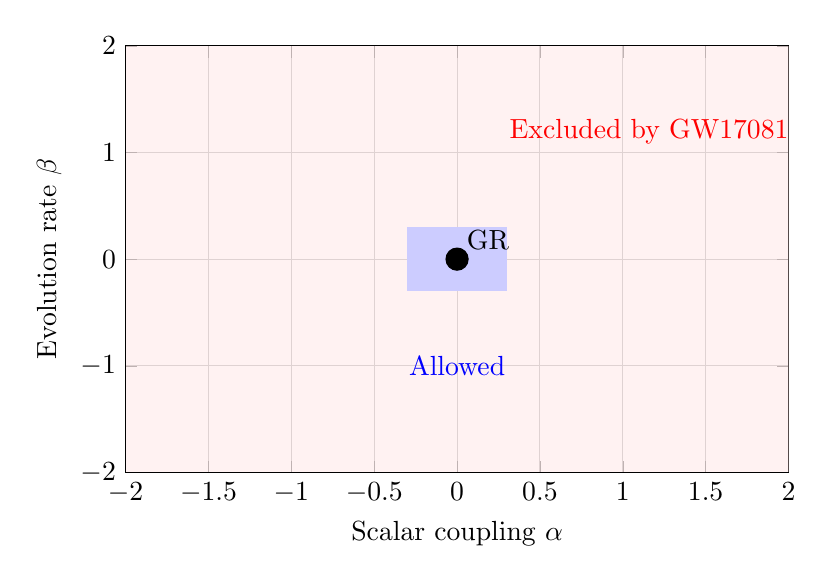
\begin{tikzpicture}[scale=1.0]
    % Constraints from GW170817 on scalar-tensor parameter space
    \begin{axis}[
      width=10cm, height=7cm,
      xlabel={Scalar coupling $\alpha$},
      ylabel={Evolution rate $\beta$},
      xmin=-2, xmax=2,
      ymin=-2, ymax=2,
      grid=major,
      colormap/viridis
    ]
      % Allowed region (small patch near origin)
      \fill[blue!20] (axis cs:-0.3,-0.3) rectangle (axis cs:0.3,0.3);

      % Excluded region (everything else)
      \fill[red!10,opacity=0.5] (axis cs:-2,-2) rectangle (axis cs:2,2);
      \fill[blue!20] (axis cs:-0.3,-0.3) rectangle (axis cs:0.3,0.3);

      % GR point
      \addplot[mark=*,only marks,mark size=4pt,black] coordinates {(0,0)};
      \node[above right] at (axis cs:0,0) {GR};

      % Labels
      \node at (axis cs:1.2,1.2) {\textcolor{red}{Excluded by GW170817}};
      \node at (axis cs:0,-1) {\textcolor{blue}{Allowed}};
    \end{axis}
  \end{tikzpicture}
  \caption{Constraints on scalar-tensor theories from gravitational wave speed. The red region is excluded by GW170817 + GRB 170817A, which measured $c_T = c$ to $10^{-15}$ precision. Only a tiny blue region near GR ($\alpha = \beta = 0$) remains allowed. Most Horndeski models are ruled out.}
  \label{fig:p4:gw-constraints}
\end{figure}

%------------------------------------------------------------------------------
\section{Chapter Summary and Forward Bridge}
\label{sec:p4:scalar-tensor-summary}
%------------------------------------------------------------------------------

This chapter developed the mathematical framework of scalar-tensor gravity, from action principles through field equations to observational constraints.

\marginhistory{From Jordan's 1955 question "Is gravity variable?" to the 2017 GW170817 observation spans 62 years of theoretical development and experimental refinement.}

\textbf{Key results:}
\begin{enumerate}
  \item \textbf{Two frames}: Jordan (equivalence principle) vs Einstein (standard GR + scalar) are conformally related
  \item \textbf{Modified dynamics}: Scalar field mediates fifth force, couples to matter trace $T$
  \item \textbf{Tight constraints}: Solar system tests require $\omega > 40,000$ (Cassini); GW speed requires $|c_T - c|/c < 10^{-15}$
  \item \textbf{Screening mechanisms}: Chameleon and Vainshtein allow large cosmological effects while satisfying local bounds
  \item \textbf{$f(R)$ equivalence}: Any $f(R)$ theory maps to scalar-tensor with specific $\omega(\phi)$ and $V(\phi)$
\end{enumerate}

\textbf{Observational status (2025):}
\begin{itemize}
  \item No confirmed deviations from GR in solar system or gravitational waves
  \item Scalar dark energy (quintessence) remains viable but not required by data
  \item Screened models can explain dark energy while satisfying all tests
\end{itemize}

\marginphysics{The scalar field $\phi$ mediates gravity-matter coupling. In Chapter 3, we extend this to gravity-EM coupling, where $\phi$ connects metric curvature to electromagnetic fields.}

\textbf{Forward to Chapter 3:}

Having established scalar-tensor gravity, we now investigate electromagnetic coupling. The scalar field $\phi$ can mediate interactions between gravitational curvature $R$ and electromagnetic field strength $F_{\mu\nu}$. We derive coupling mechanisms, analyze Reissner-Nordstr\"om charged black holes, and examine how electromagnetic stress contributes to spacetime curvature. This sets the stage for the full unified field equations in Chapter 4.

%==============================================================================
% END OF CHAPTER 2
%==============================================================================
